\documentclass[12pt,a4paper]{article}

%language and font
\usepackage[utf8]{inputenc}
\usepackage[english]{babel}
\usepackage[scaled]{beramono}
\usepackage[T1]{fontenc}

%% Useful packages
\usepackage{pdfpages}
\usepackage{amsmath}
\usepackage{mathrsfs}
\usepackage{amssymb}
\usepackage{graphicx}
\usepackage[colorinlistoftodos]{todonotes}
\usepackage[colorlinks=true, allcolors=blue]{hyperref}
\usepackage[left=2cm,right=2cm,top=2cm,bottom=2cm]{geometry}
\author{Y1471938}
\title{

\includegraphics[width=\textwidth]{images/yorkUniLogo.png}\\
\textbf{Systems programming for ARM}\\ extending DocetOS}

\begin{document}
\maketitle
\begin{abstract}
This document outlines the extensions and modifications made to the DocetOS operating system. The focus of the extensions is on scalability with the aim of allowing the extended docetOS to work with a large number of tasks efficiently. This results in a slight overhead in memory usage but allows for a stochastic priority scheduler that can efficiently switch between many tasks, and prevent starvation of individual tasks by ensuring that even the lowest priority task gets occasionally allocated CPU time. The scheduler incorporates an efficient task sleeping and waiting mechanism which aims to minimise the operations that have to be performed when a task transitions from one state to another. I have provided the user with tools to easily set up inter task communication through the OS channel manager, which is responsible for providing one or more tasks with access to the correct channel, and recycling the channel once the tasks no longer need it. In order to allow the user to easily allocate memory I have created a "memory cluster" that simultaneously aims to prevent memory being wasted and tasks having to wait for memory to become available. The memory provided by the cluster is guaranteed to be 8-byte aligned and can therefore also be used for task stacks. The OS itself uses the memory cluster to allocate the vast majority of its own internal resources such as hash tables, queues, heaps etc. All data structures used by the OS are standalone and available to the user for their own use. They come with convenience functions to quickly create and destroy them e.g "new\_hashtable(...)" allocates and initialises a hash table with the desired size. To prevent priority inversion the operating system supports priority inheritance for tasks using the mutex struct that comes with the OS.
\end{abstract}
\pagebreak
\tableofcontents
\pagebreak
\section{The Stochastic Scheduler}
My plan was to allow DocetOS to support a large number of tasks, which made me come up with the following key requirements for the priority scheduler:
\begin{itemize}
  \item The scheduler should be pre-emptive, but allow tasks enough time to run to avoid wasting CPU time on frequent context switching.
  \item CPU time allocated per task should be dependant on the tasks priority, but the highest priority task should not be the only task getting CPU time (not just standard Fixed priority pre-emptive scheduling behaviour where only the highest priority task is selected)
  \item Task starvation should be avoided, even the lowest priority task should have a non-zero probability of getting selected during task switch.
  \item Task switching and status changes of tasks should not result in a large overhead of CPU time.
    \item The scheduler needs to avoid priority inversion.
\end{itemize}

\pagebreak
\subsection{Implementation}
At the end of this section you will find an example illustration of the internal state of the scheduler at a particular point in time. The scheduler contains 2 heaps and 5 hashtables which are used to keep track of the various states a task can be in, and allow quick access to any task no matter its state.

\begin{itemize}
  \item The \textbf{Scheduler Heap} is used by the scheduler to determine what task to select for execution. This heap can contain tasks that are active and tasks that are waiting, sleeping or have tasks that have run to completion (see highlight 1). Tasks that are not active are only moved/removed from the scheduler heap if they are encountered in the heap during task selection. This is done to save cpu time on operations that might be unnecessary, a task that goes to sleep might wake up long before the scheduler comes across it in the heap, so moving it to the sleep heap would only waste cpu cycles on restructuring the sleep and scheduler heaps. When the scheduler comes across a sleeping/waiting task it checks if this state is still applicable and only then moves the task to a different heap/hashtable.
  \item The \textbf{Sleep Heap} stores tasks that are sleeping and have been removed from the scheduler heap. In this heap the tasks position in the heap is not determined by its priority but by its remaining sleep time (highlight 2). The scheduler removes the first node, updates its remaining sleep time by referring to the time it started sleeping and checks if it has woken up, if it has it is added back to the scheduler heap and the process is repeated. If the first node has not woken up yet then none of the other nodes will have woken up either. This approach means only one sleeping node has to be updated.
  \item The \textbf{tasksInSchedulerHeapHashTable} keeps track of all the tasks currently present in the scheduler heap. Used to check what tasks have to be added back to the scheduler heap after wake/notify and which ones were never removed.
  \item The \textbf{activeTasksHashTable} keeps track of all tasks that are currently executable.
  \item The \textbf{waitingTasksHashTable\_reasonAsKey/\_tcbAsKey} both keep track of tasks that are waiting. The \_reasonAsKey table is used during notify to change the state of a task waiting for "reason" without needing to check each waiting task. the \_tcbAsKey allows the OS and user to check if a given task is waiting.
  \item The  \textbf{sleepingTasksHashTable} keeps track of all tasks that are sleeping, no matter what heap they are in.
  \item The  \textbf{nodeContentIndexHashTable} internal (optional) hashtable of heap data structure, can be used to quickly determine at what index a node with a specific content is located in the heap. This is used during priority inheritance.
\end{itemize}

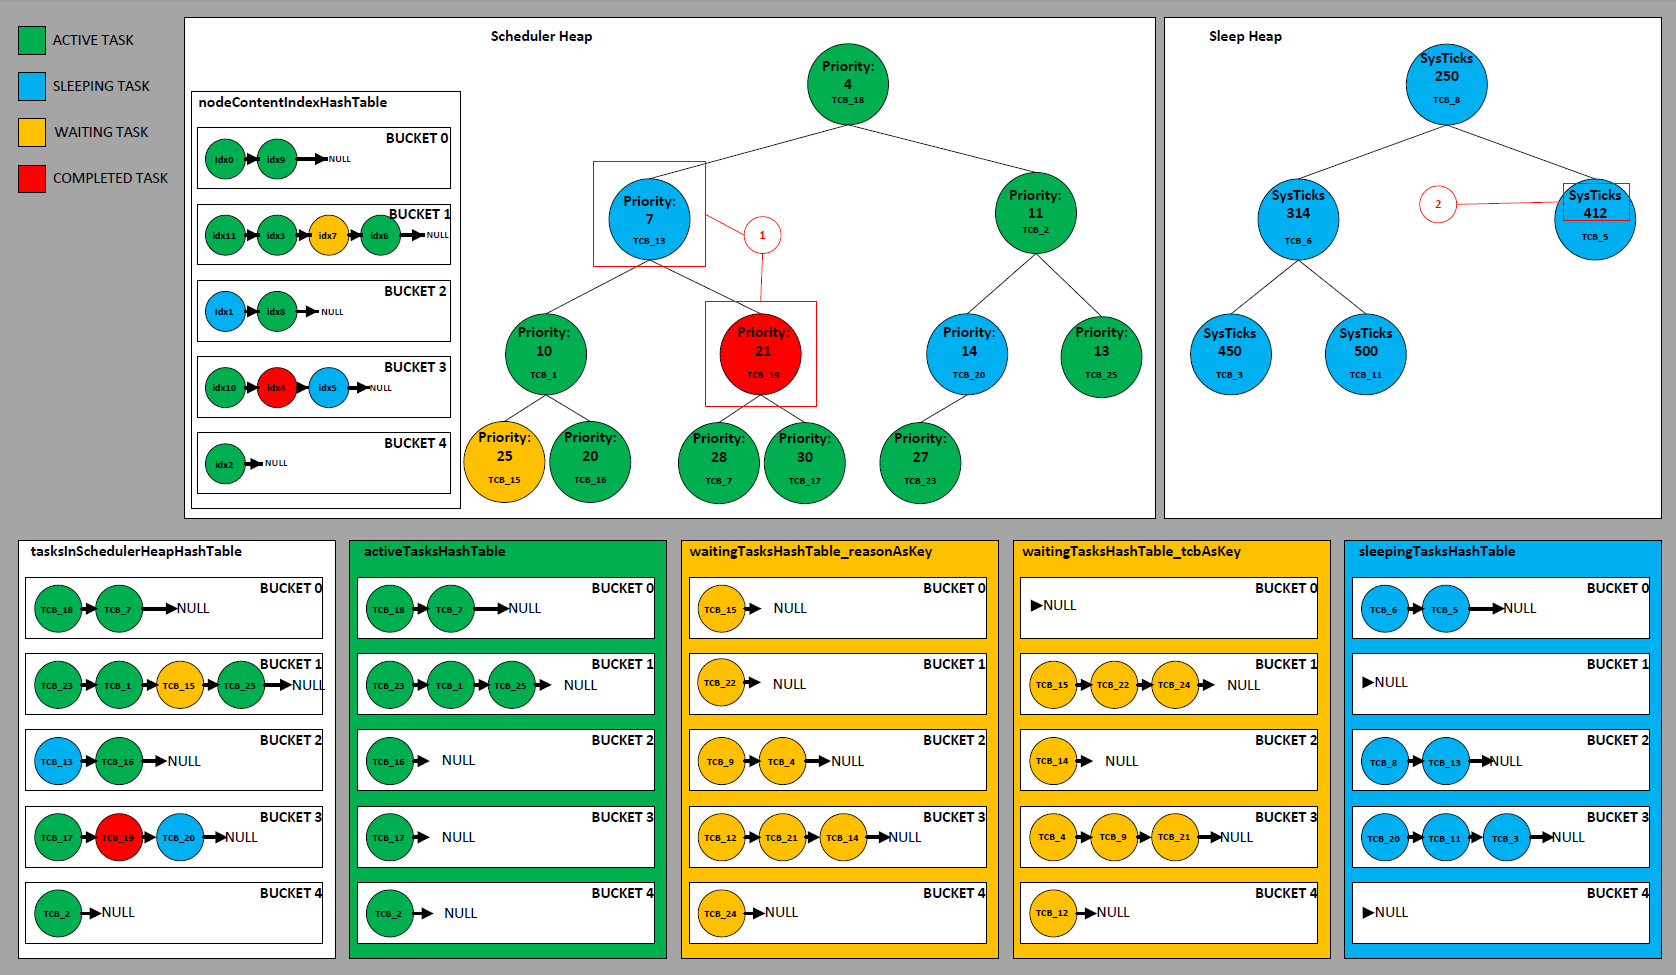
\includepdf[landscape=true]{images/schedulerOverview.png}


\subsection{Selecting a Task}
Before a task switch is initiated the scheduler checks if the current task has changed state (from active to sleep, wait etc.) or if it has exceeded its maximum runtime (set in the scheduler header). The scheduler does not force a task switch every SysTick to avoid wasting cycles on the task selection process. The scheduler task selection process uses a min heap which stores the tasks in ascending order of priority (lower number means the task has a higher priority). Starting from the top node of the heap the scheduler decides at each node (via pseudo random number) if the current node should be selected or if the process should be repeated for one of the child nodes. If during this process the scheduler comes across a task that is not in the active state it will remove it from the scheduler heap and place it in the corresponding heap/hashtables. The reason for not removing a task instantly when it goes into the sleep or wait state is that the task could wake/get notified before the scheduler encounters it during task selection, which would mean that moving it from the scheduler heap would have just wasted cycles.\\

The reasoning behind using a heap and an element of randomness for task selection (with the chance of a task getting selected being correlated with the tasks priority) is that it avoids task starvation by giving every task a non-zero probability of getting selected, no matter how low their priority. My heap data structure also has a modification that the user can enable which allows the heap to store the index where certain content can be located in the heap, this allows for quick insertion/removal of nodes at any heap index. This is especially useful during priority inheritance process. 
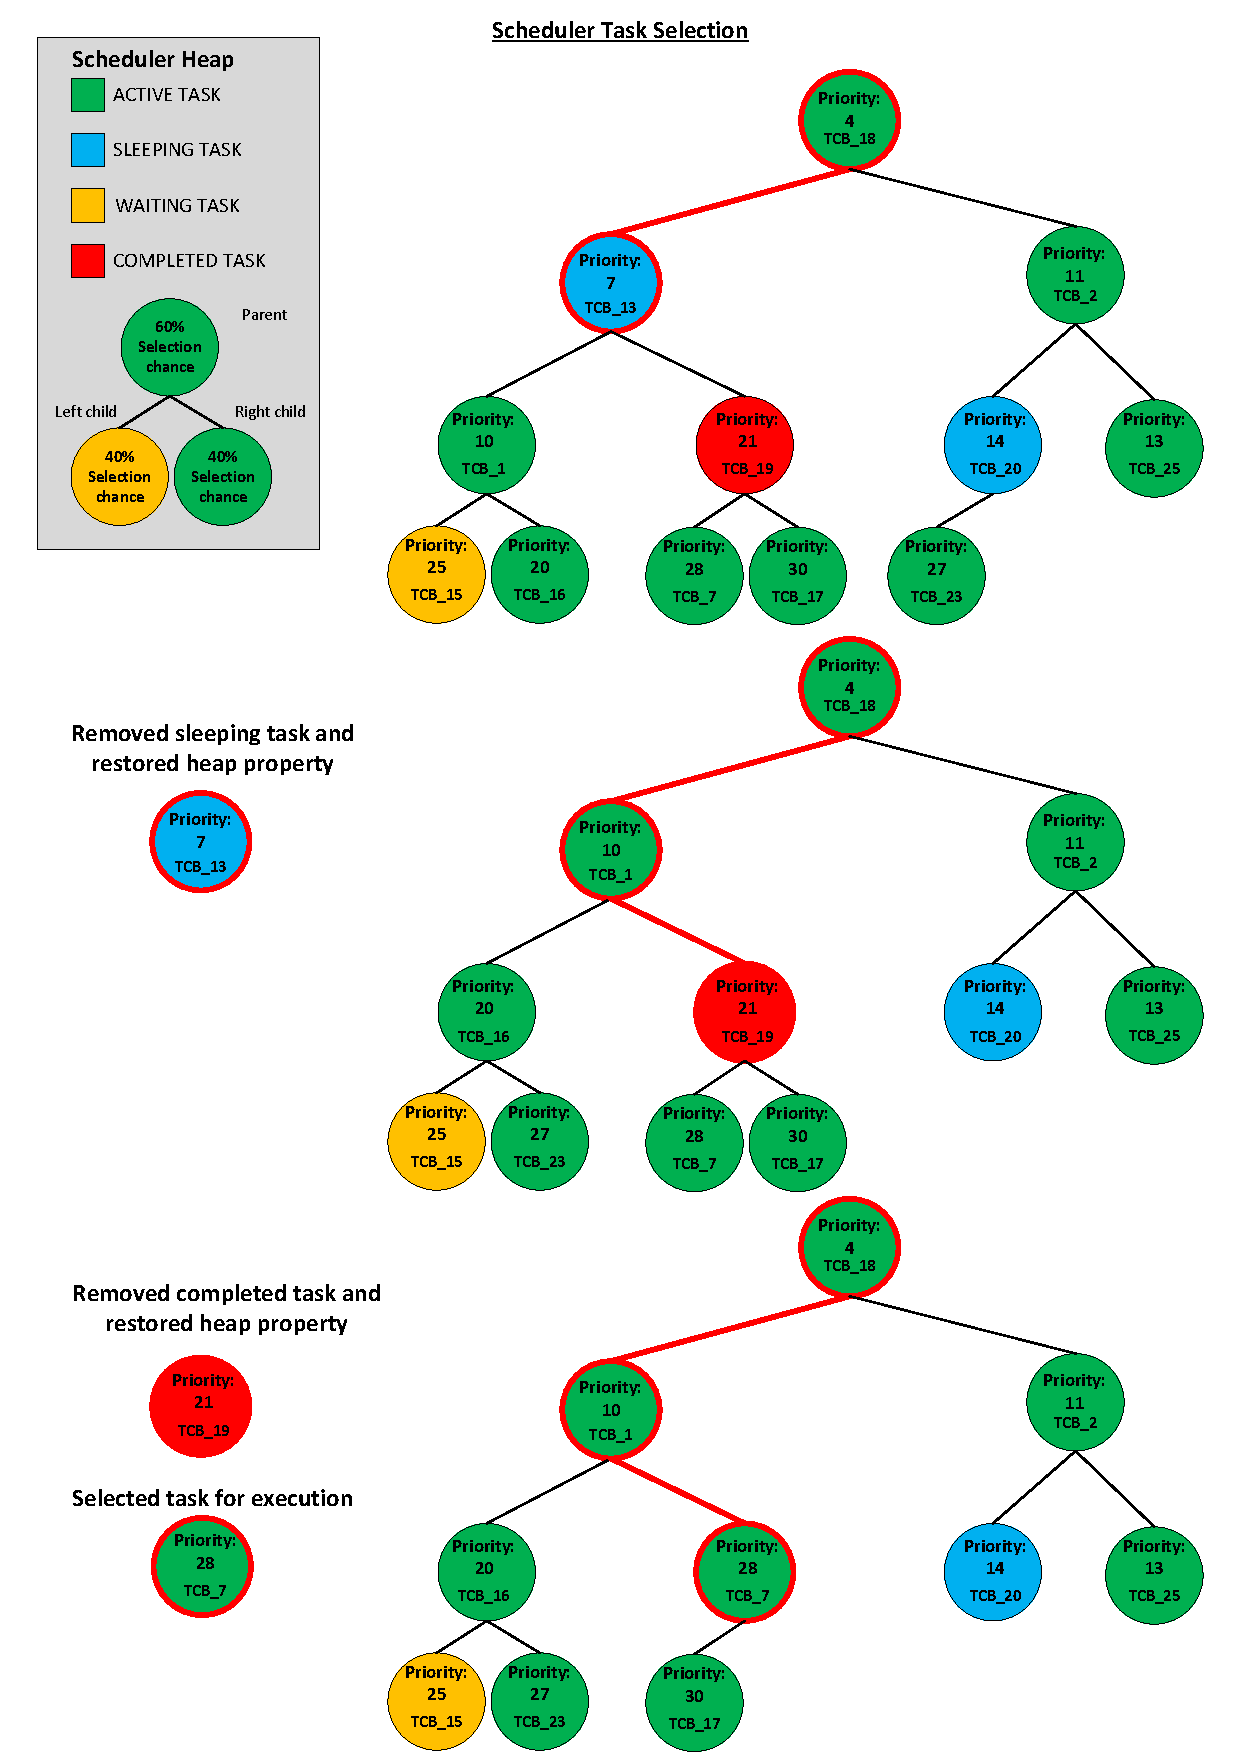
\includepdf[scale=0.9,pages=1]{images/schedulerTaskSelection.pdf}
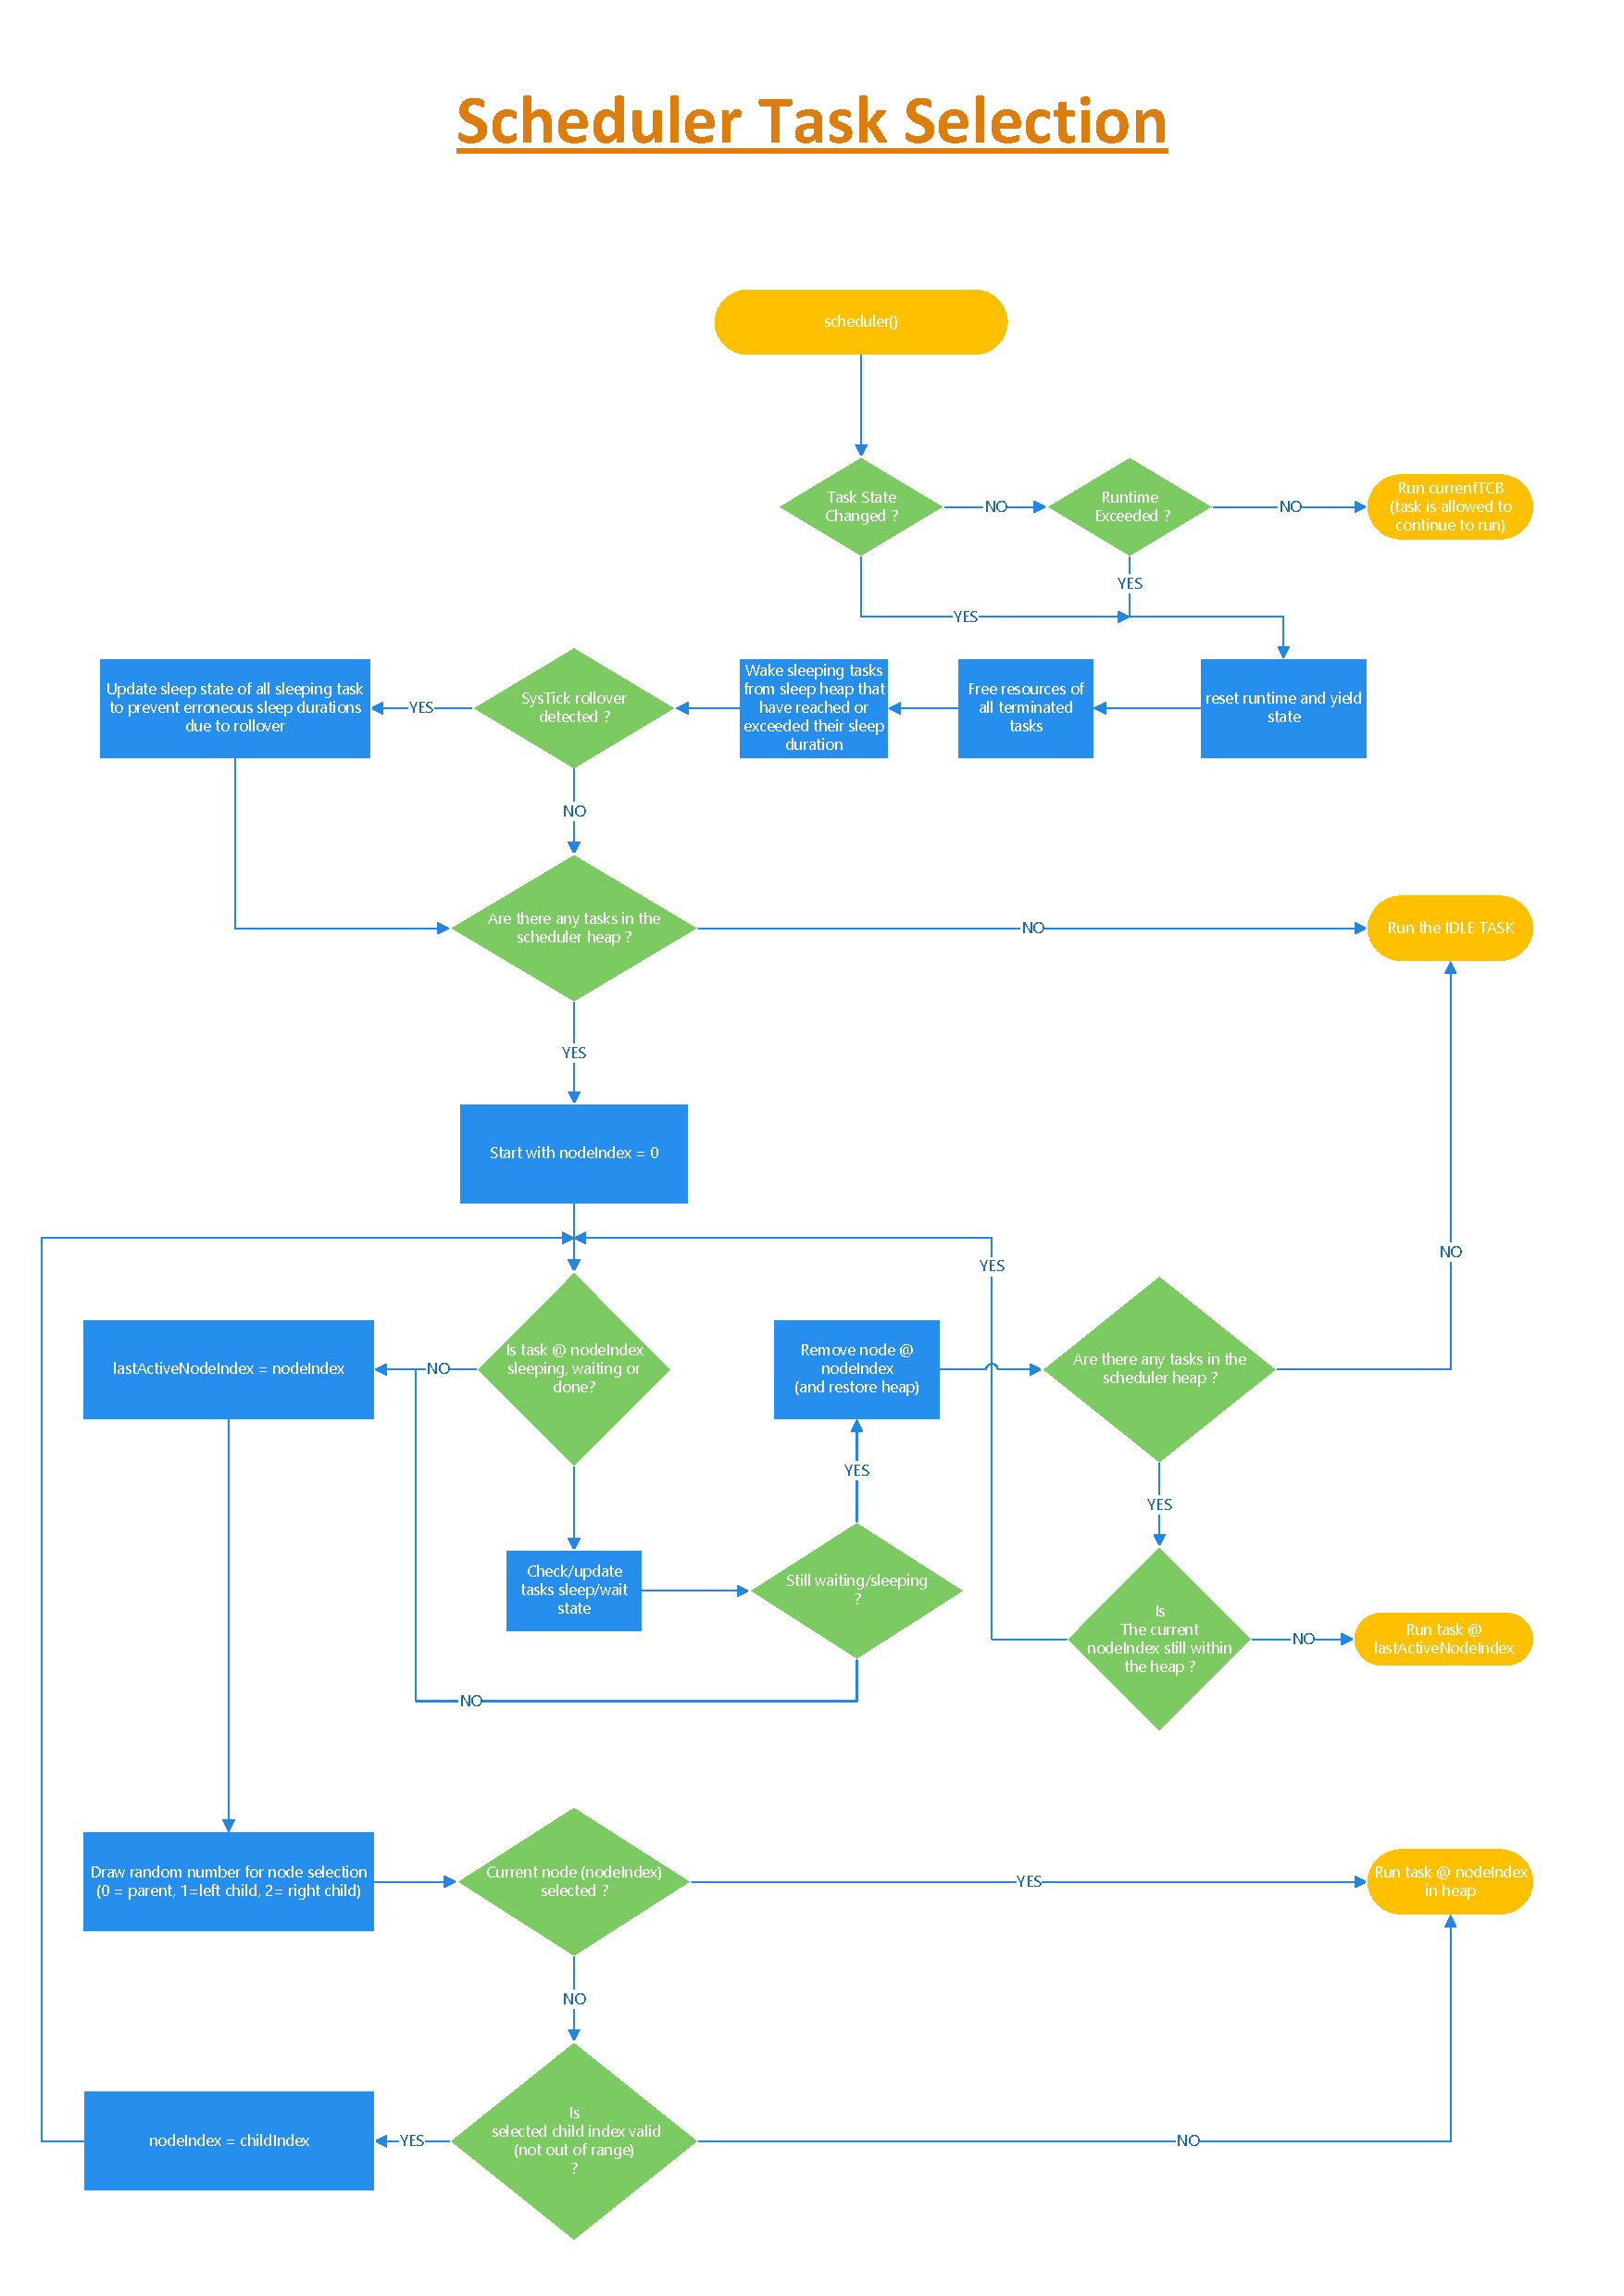
\includepdf[scale=0.9,pages=1]{images/SchedulerTaskSelectionFlow.pdf}
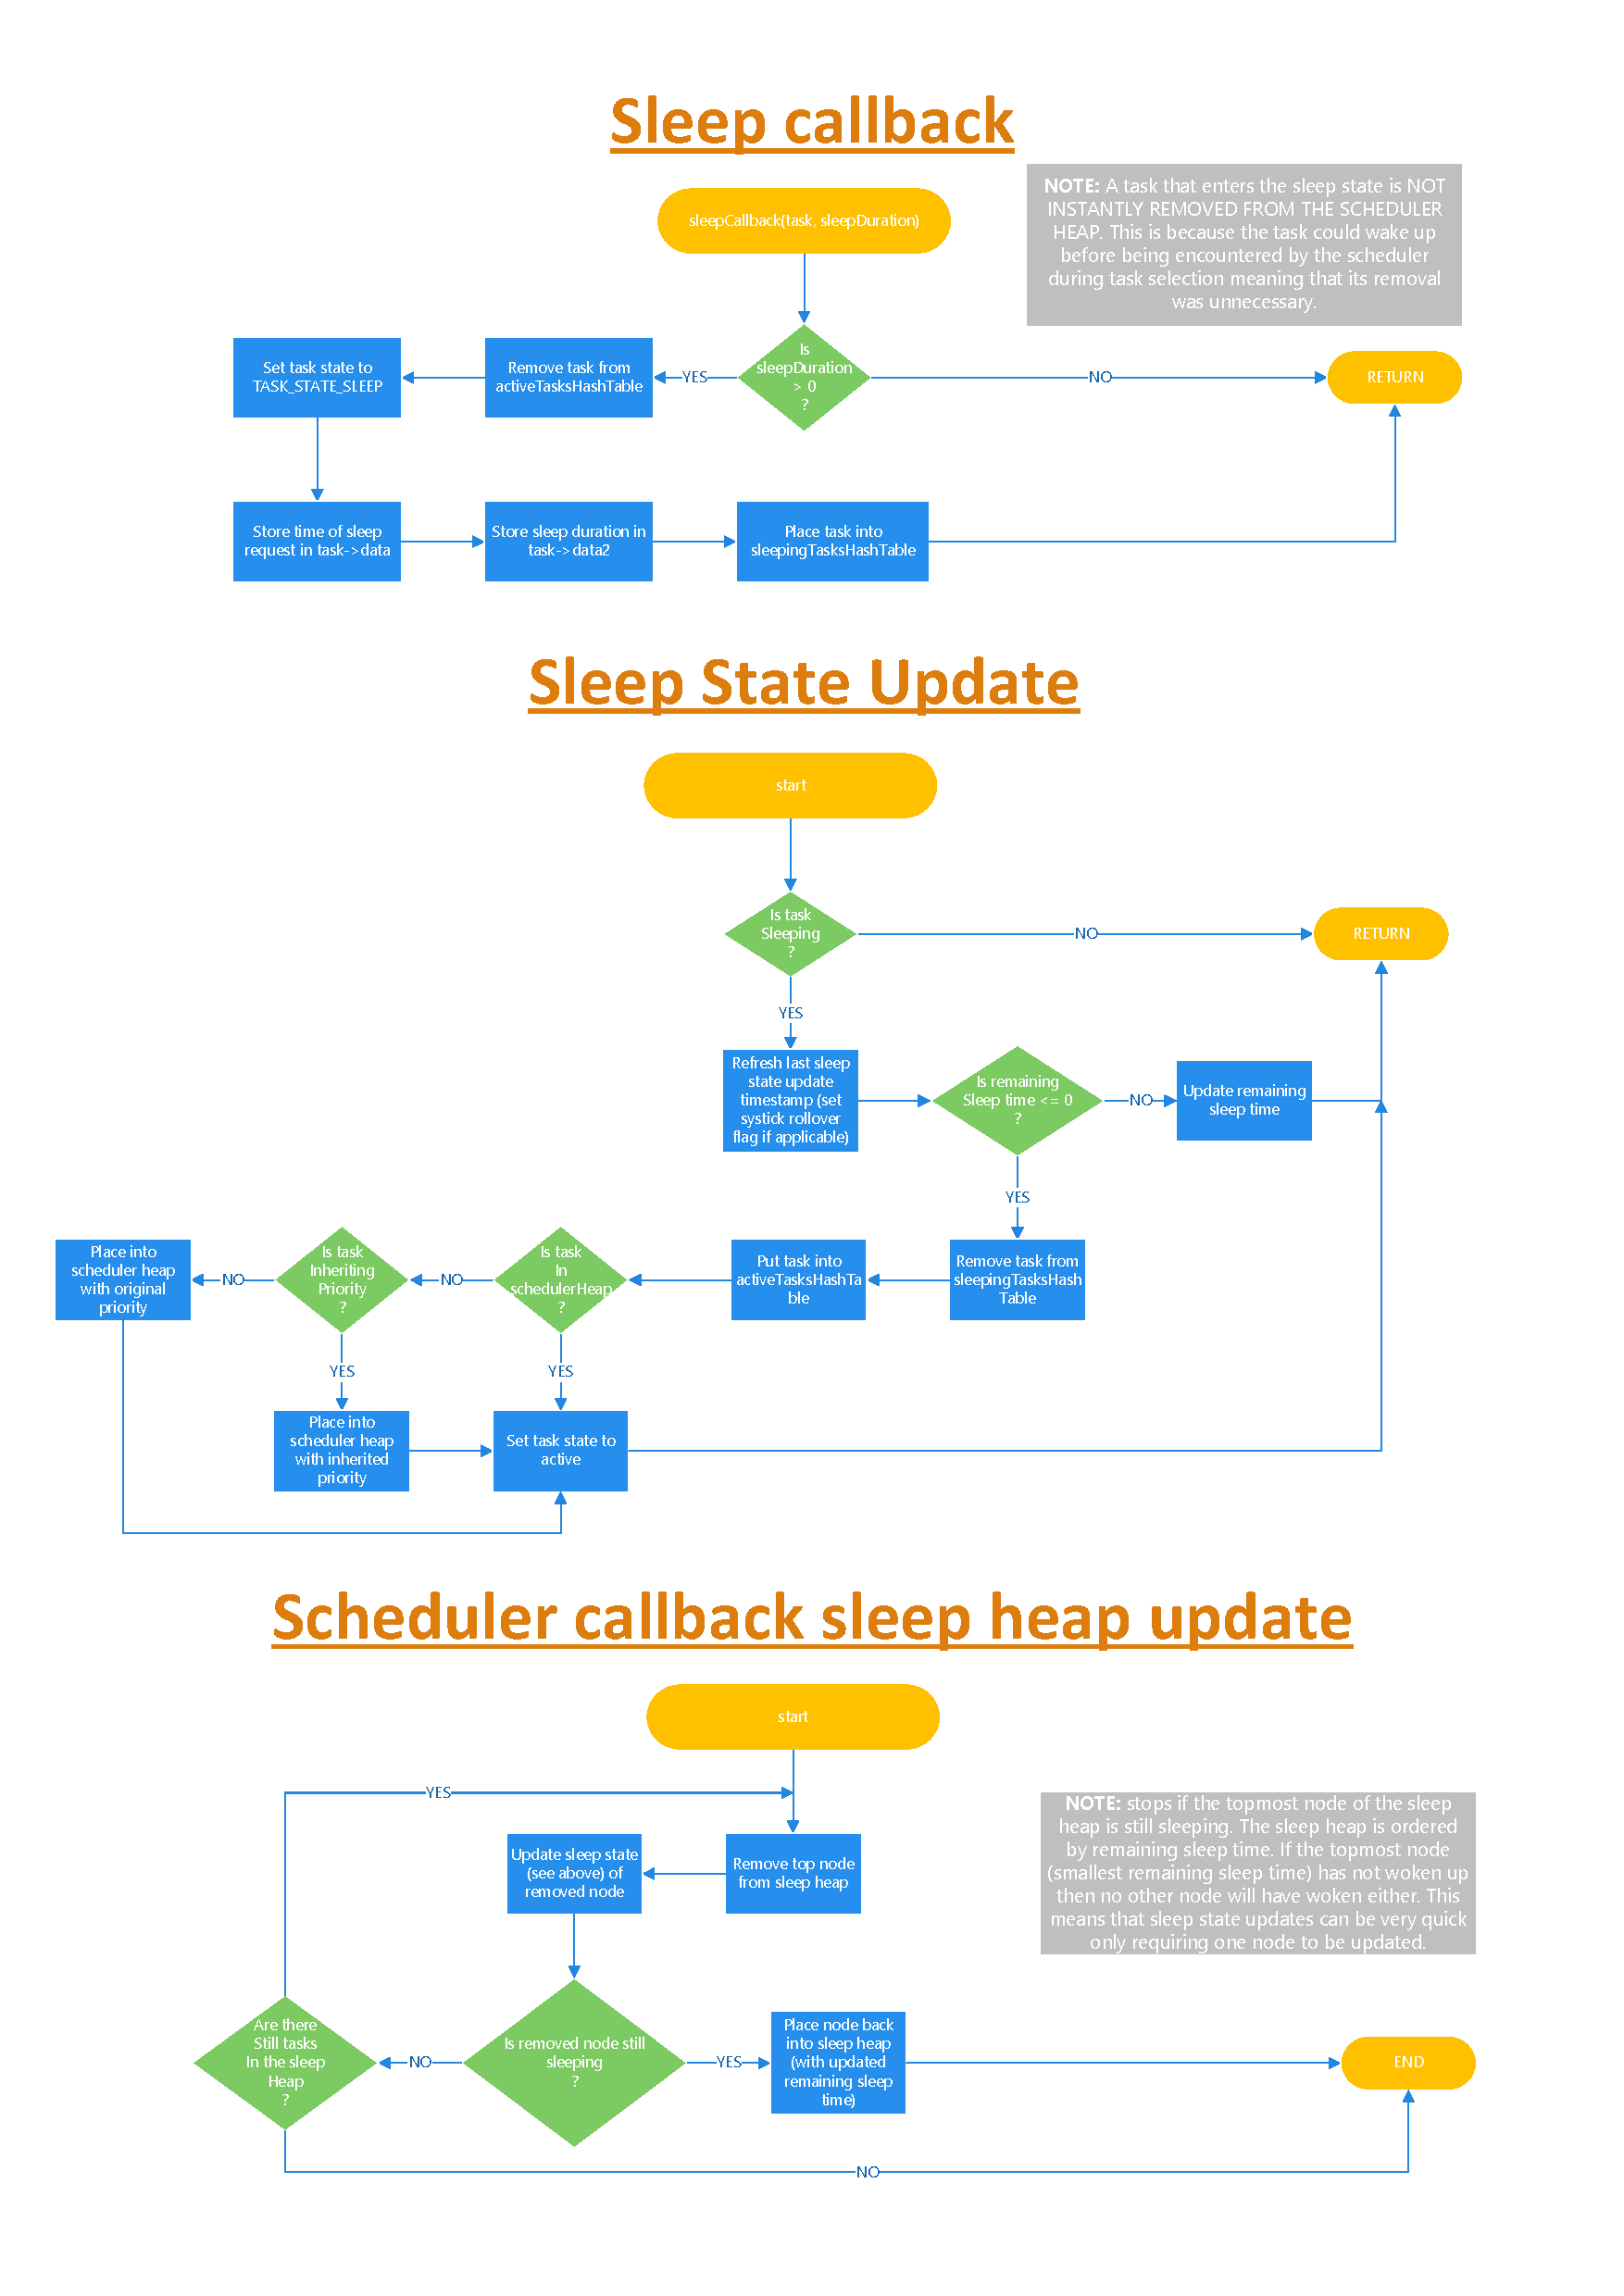
\includepdf[scale=0.9,pages=1,pagecommand=\subsection{Sleep}]{images/SchedulerSleep.pdf}
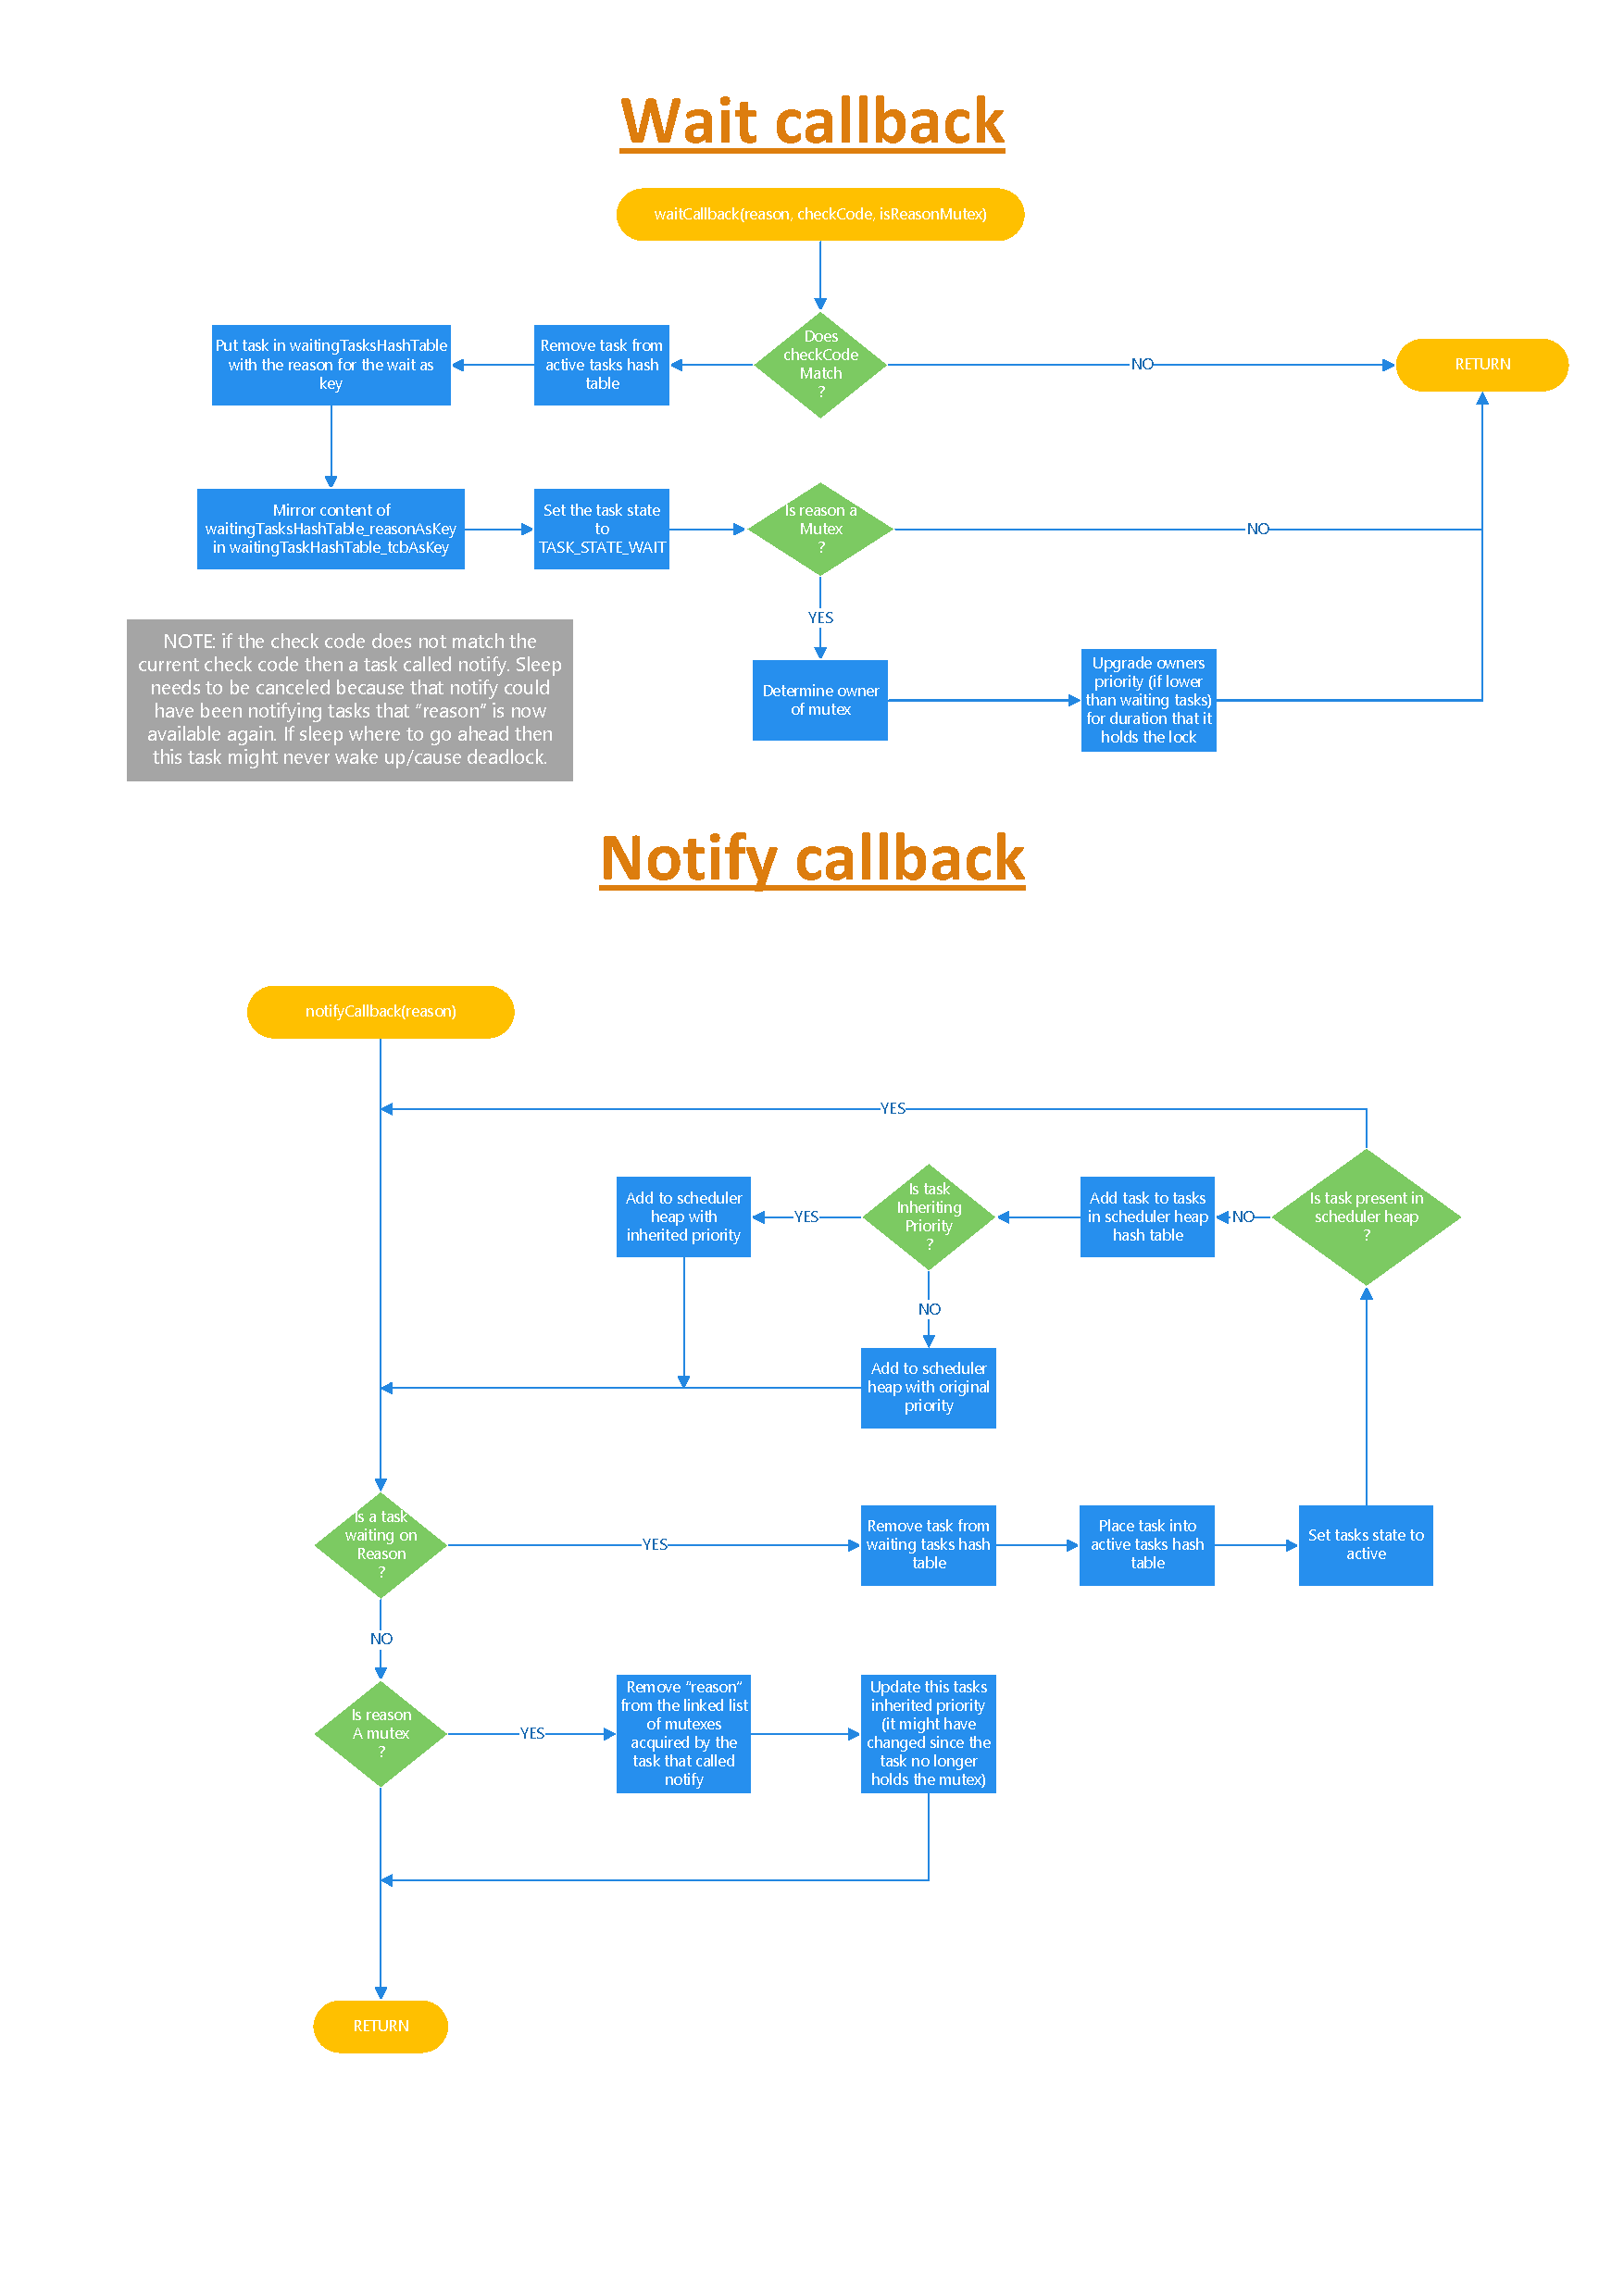
\includepdf[scale=0.9,pages=1,pagecommand=\subsection{Wait and Notify}]{images/WaitNotifyFlow.pdf}
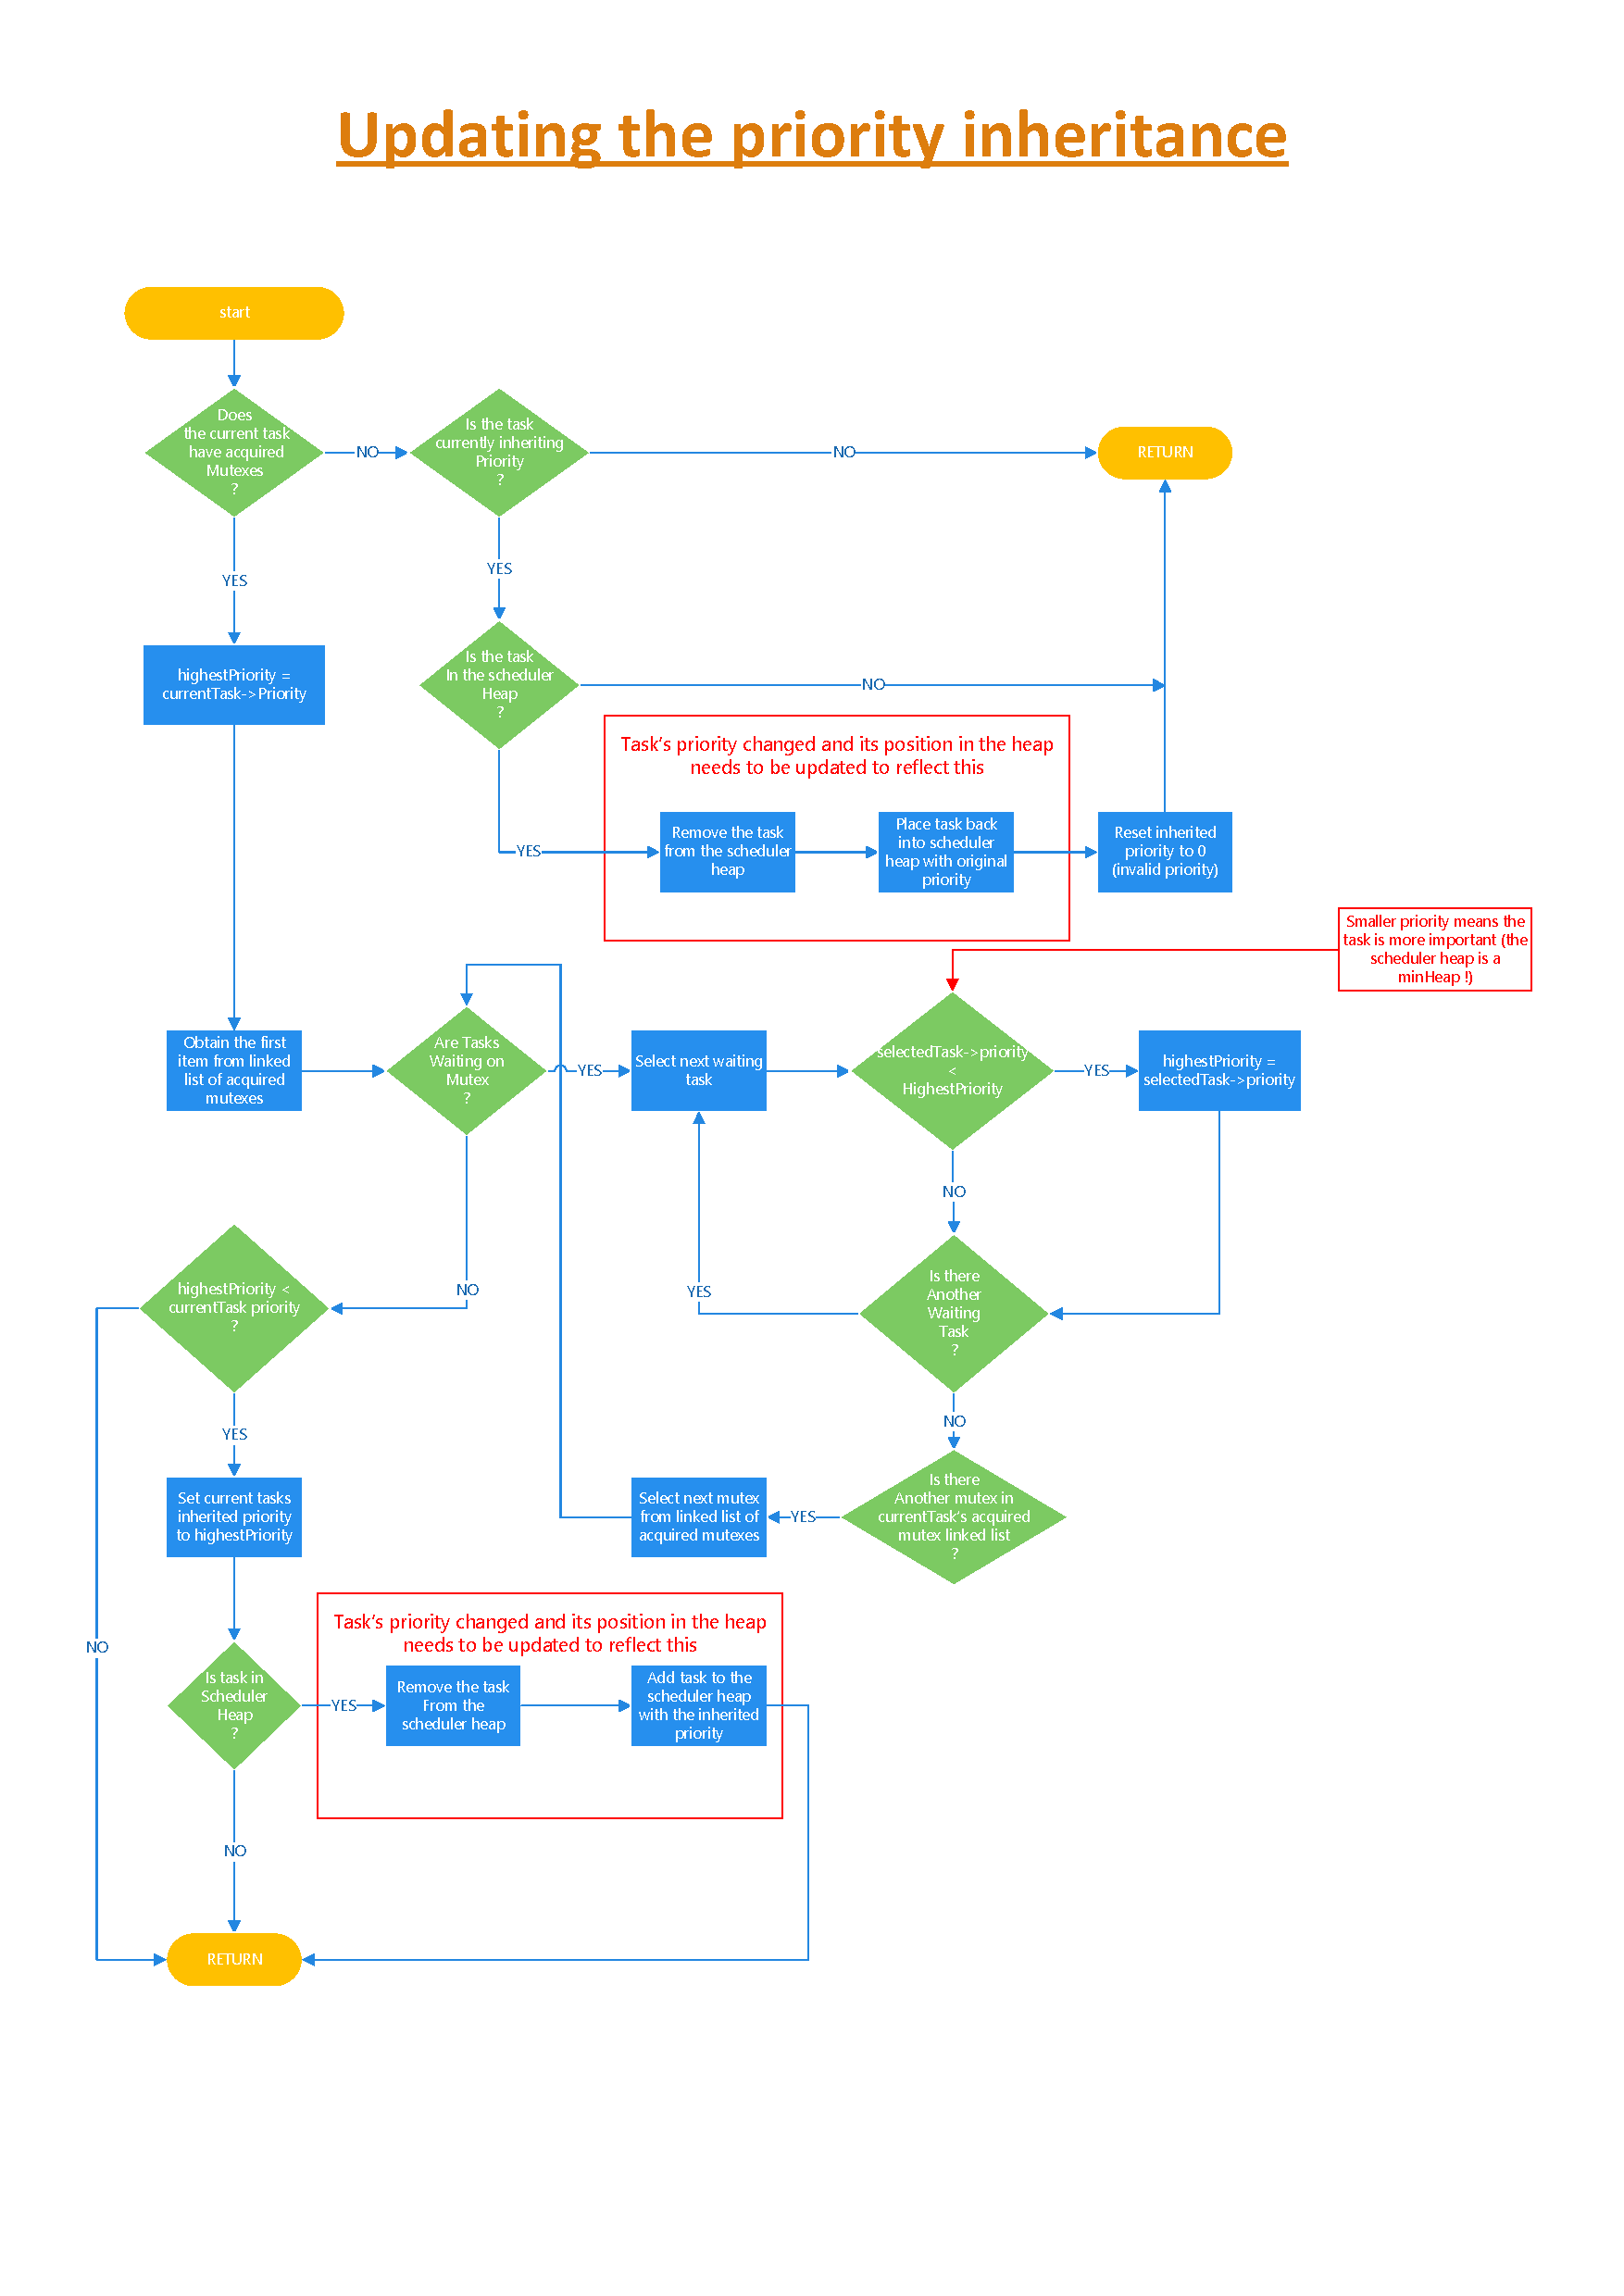
\includepdf[scale=0.9,pages=1,pagecommand=\subsection{priority Inheritance}]{images/PriorityInheritanceFlow.pdf}

\section{The Memory Cluster}

\subsection{Design Overview}
\subsection{Initialisation Process}
\subsection{Internal Resources}

\section{The Channel Manager}
\subsection{Design Overview}
\subsection{The Channel}
\subsection{Initialisation Process}

\section{Data Structures}
\subsection{Mutex}
\subsection{Semaphore}
\subsection{Queue}
\subsection{Hashtable}
\subsection{Heap}

\pagebreak
\section{Demonstration Code Overview}
The demonstration code contains 14 tasks that together highlight the various features of the modified OS. The demonstration begins with the creation and initialisation of a single task (task0). All task resources are allocated using the memory cluster. This is possible because the memory cluster guarantees that the memory blocks it returns are 8-byte aligned. The OS is then started and task 0 begins its execution. It allocates, initialises and adds 9 further tasks to the scheduler from within the running task itself. After this task0 exits and the resources associated with it (TCB and stack) are deallocated by the OS. Below this paragraph you can see an annotated screen shot of the demo output. The screenshot shows the state of the counter of each of the tasks. The bracketed red numbers indicate which task holds the print Lock and executed the printf.\\

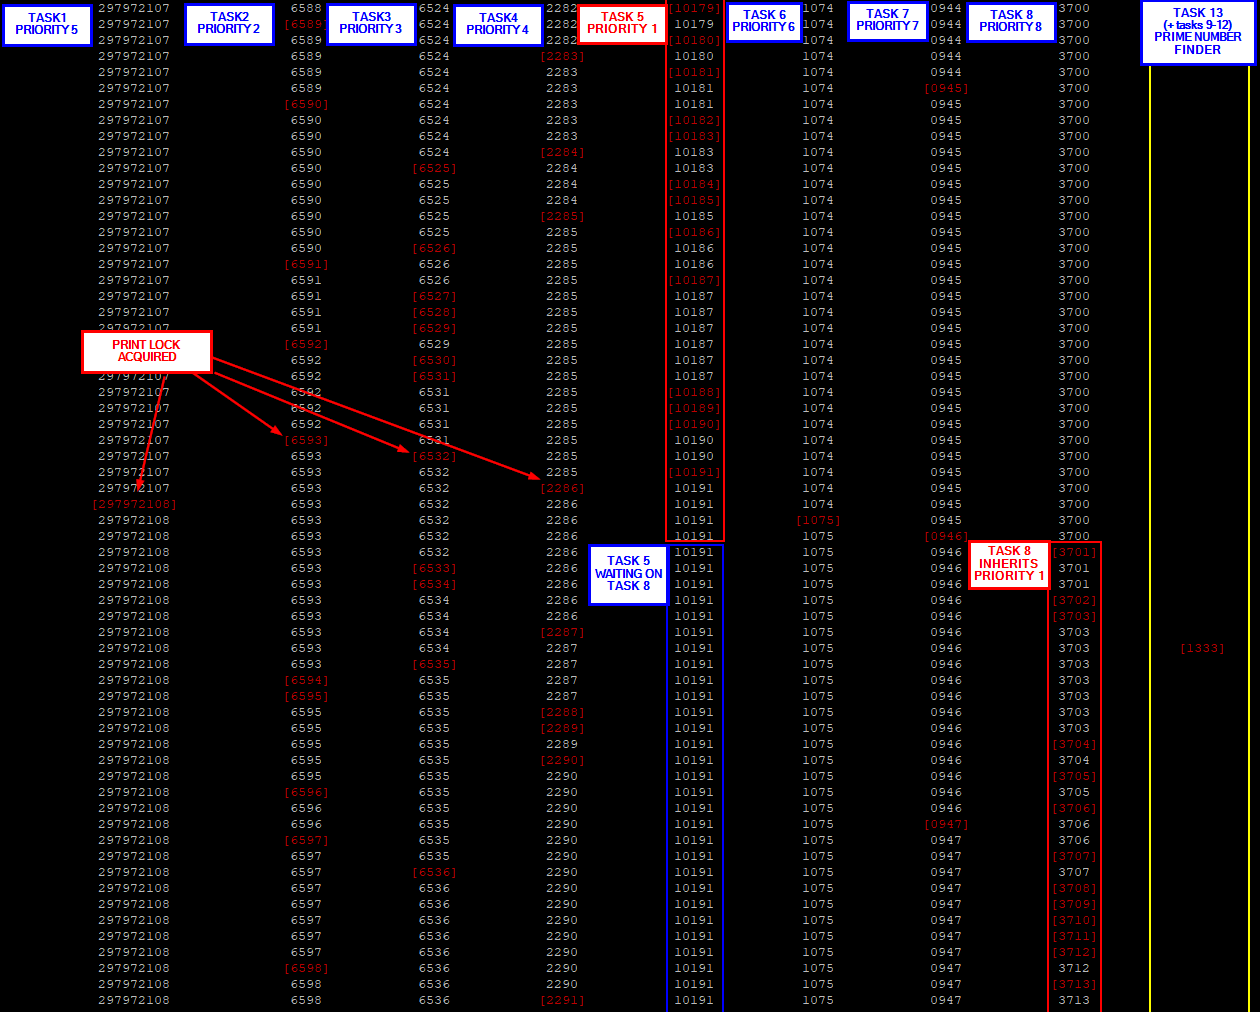
\includegraphics[width=\textwidth]{images/priorityInheritance.png}\\

Tasks 1 through 4 and tasks 6 and 7 demonstrate the operation of the mutex datatype. Task 1 is an exception because rather than wait whilst another mutex owns the lock it uses the OS\_mutex\_acquire\_non\_blocking function which enables it to skip the printf section if it is not successful in obtaining the lock because another tasks holds it. This allows it to continue increasing its counter when other tasks would have to wait. By inspecting the count that tasks 2,3,4,6 and 7 have obtained in the screen-shot and comparing this count to their priorities it can be seen that cpu time allocated to the task is dependant on the task's priority. The screen-shot also highlights that the scheduler does not only allocate time to the highest priority task and thereby prevents task starvation of lower priority tasks (see how task 4 with priority 4 still occasional increases its count despite task 5 with priority 1 also being active).\\

Task 5 and 8 demonstrate the schedulers priority inheritance functionality. Priority inheritance is a feature that prevents a condition known as priority inversion where a lower priority task can potentially starve a higher priority task. This is avoided by giving the lower priority task the priority of the higher priority task for the duration that the lower priority task holds the lock to a shared resource that both tasks use. \\

Task 13 (spawned from task0) is an implementation of the Sieve of Eratosthenes prime number finding algorithm which I use here to demonstrate the inter task communication abilities of the OS. The OS allows task to communicate using channels. A task can obtain a channel from the OS channel manager by stating a channel ID (the user can also create and use channels not managed by the channel manager if they so desire). Two tasks that request the same ID both get given the same channel which they can now use to pass data back and forth. The use of the channel manager lets tasks create and use channels dynamically rather than the user having to create all channels beforehand (the channel manager uses the OS memory cluster for channel allocation). Task13 allocates, initialises and adds task 9-12 to the scheduler, it also creates 4 distinct channels. Tasks 9-12 connect to one channel each. task 9 has a counter starting at 2, all numbers where (num \% 2 == 0) get written to the channel it shares with task 13. tasks 10,11 and 12 do the same with 3,5 and 7 respectively. task13 reads from the 4 channels and compares the number. If all 4 numbers match then it shows that that number is a prime and task 13 prints it to the serial bus.

\end{document}